\section{Tag rate function method}
\label{chp:sec:trf}

The estimation of backgrounds at high $b$-tag multiplicity can be challenging if MC statistics is fairly low, especially for those samples that are selected because of light-jet mistags (mistag rate $<1\%$). Analyses that use the shape information to extract the signal can be negatively affected by the large statistical uncertainties on the templates and unreliable systematic uncertainties due to shape fluctuations. The tag rate function (TRF) method \cite{Shibata:1042972,TRF} helps increase the effective statistics of the MC samples by using all the events prior to the $b$-tag selection and weighting, rather than rejecting, those events not containing the specific number of $b$-tagged jets in simulation. The weight is computed by combining the tagging probabilities of each jet in the event. For events with a large number of $b$-jets, the method effectively compensates for the statistics losses due to $b$-tagging efficiencies. To achieve this, the tagging efficiency is parametrised as function of $\pt$, $\eta$ and truth jet flavour,\footnote{The true jet flavour is defined by looking at hadrons with $\pt > 5$ $\gev$ within a $\Delta R < 0.3$ cone around the jet direction. If a $b$-hadron is found, the jet is labelled as a $b$-quark jet. If no $b$-hadrons are found, $c$-hadrons are considered and, if found, the jet is labelled as a $c$-quark jet. If no $c$-hadrons are found either, the jet is labelled as a light-jet.} $\epsilon(\eta,p_{T},f)$ and is used to calculate the event weight based on the kinematics of the selected jets in each event. The efficiency maps used are shown in figure \ref{sec:obj:fig:btageff}.

When requiring a given number of $b$-tagged jets in the event ($n_{b}$), all permutations are built considering $n_{b}$ jets labelled as tagged among $N$ jets in the event; in total $C(N,n_{b})=\binom{N}{n_{b}}$ permutations are possible. The probability of each permutation is computed from the multiplication of the per-jet weights: the jet weight is equal to the tagging efficiency if the jet is labelled as tagged, one minus the efficiency in the opposite case. Summing the probabilities of all permutations gives the per-event TRF weight. As an example, the probability of having exactly one $b$-tagged jet in the event with $N$ jets is given by:
\be
P_{=1}=\displaystyle\sum_{i=1}^{N}\left( \epsilon_{i} \displaystyle\prod_{i\neq j} (1-\epsilon_{j}) \right),
\ee

\noindent and in general the probability for inclusive $b$-tagging selections can be computed as:
  
\be
P_{\ge1}=1-P_{=0},
\ee
  
 \noindent where $P_{=0}$ is the probability that the event contains exactly zero $b$-tags. To compute the shape of the distributions built using $b$-tagged jet information, not only the probability for a given event is required, but also the knowledge of which jets are considered as tagged when a given number of tags is assumed. This is achieved by randomly choosing one of the possible permutations based on their relative probabilities. When comparing to data, the tagging efficiencies in the formulas above are multiplied by the corresponding SFs. To propagate the effect of systematic uncertainties, the efficiencies are modified due to the change in the SFs leading to a different event probability.\par
Closure tests on MC have been performed to validate the good performance of the parametrisation, Figure \ref{fig:dat:trf:ttlight} shows the comparison between the prediction obtained with the TRF method and the direct application of the cut on the $b$-tagging algorithm output for the $t\bar{t}+$light-jets background. In a region with exactly two $b$-tags (see figure \ref{fig:dat:trf:regiontwob}) the TRF method improves the statistical error on the yields, while in a region with at least four $b$-tags (see figure \ref{fig:dat:trf:regionfourb}) it improves not only the statistical error but as well the description of the shape. Within the available statistics, the TRF method provides a good description of yields and shapes with respect to the direct application of the $b$-tagging algorithm in the analysis regions. Whenever there is a statistically-significant ($\geq 2\sigma$) discrepancy in yields between the two methods, the yields from the TRF prediction are corrected to match those of direct $b$-tagging, in order to ensure that no bias is introduced.

\begin{figure}[htb!]
\begin{subfigure}{0.5\textwidth}
  \centering
  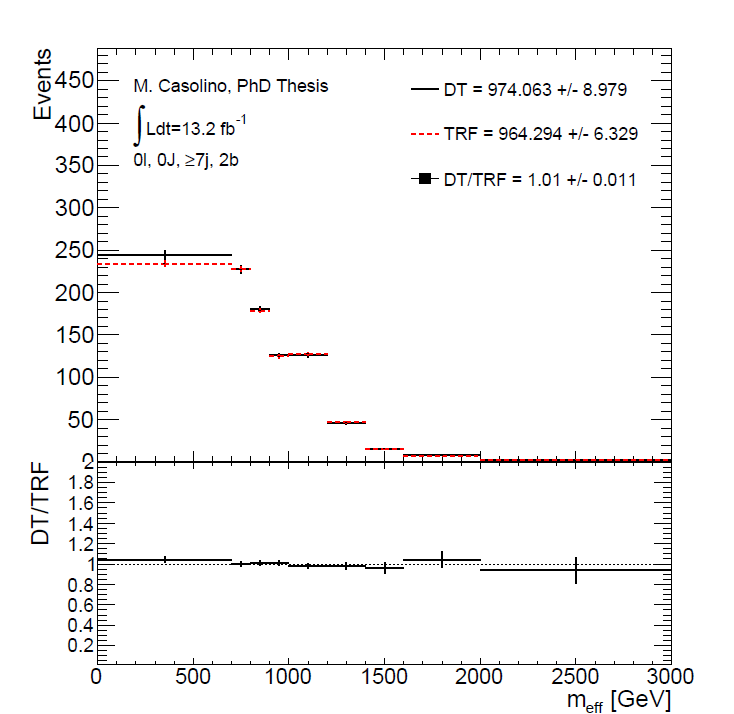
\includegraphics[width=0.9\textwidth]{figures/Datasamples/ttbarlight_meff_c0l0RCTTMass7j2b.png}
  \caption{}
  \label{fig:dat:trf:regiontwob}
\end{subfigure}
\begin{subfigure}{0.5\textwidth}
  \centering
  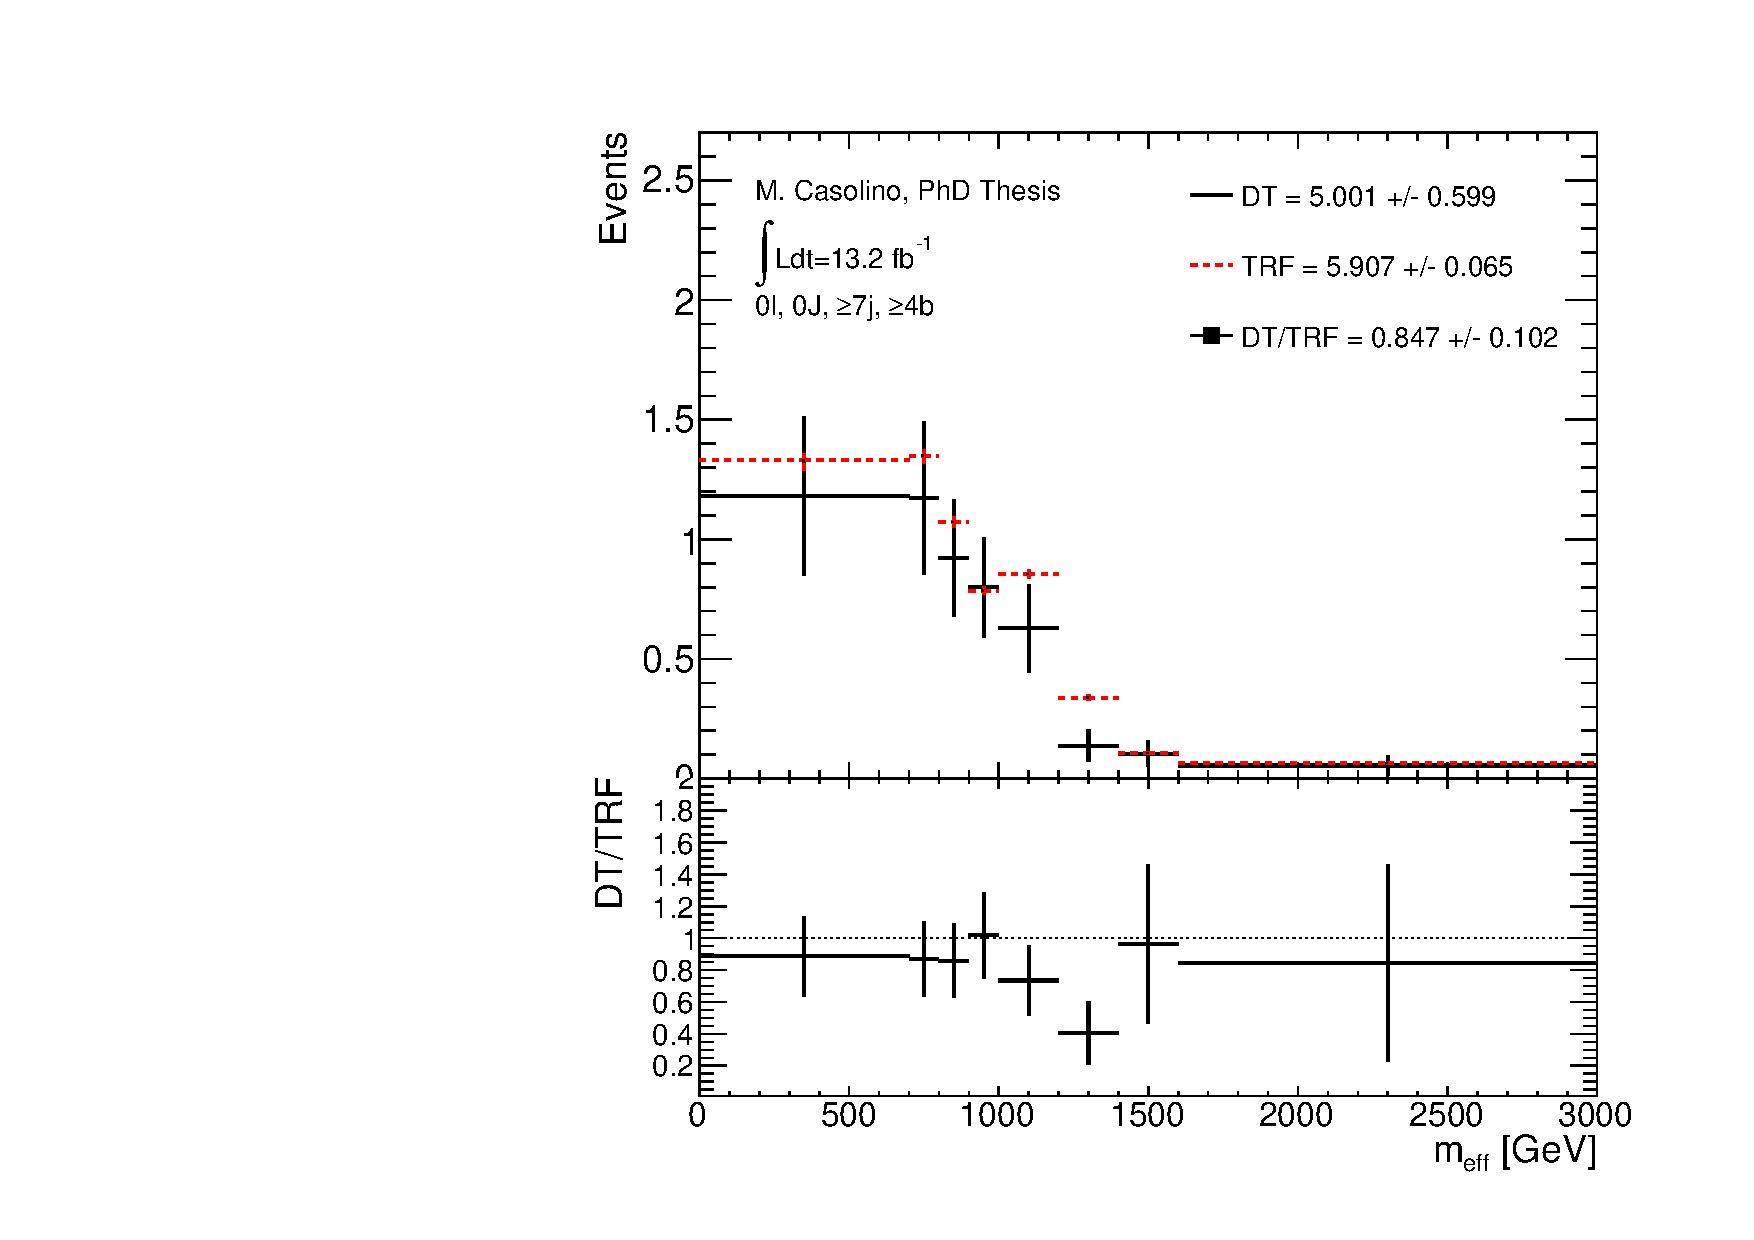
\includegraphics[width=0.9\textwidth]{figures/Datasamples/ttbarlight_meff_c0l0RCTTMass7j4b.png}
  \caption{}
  \label{fig:dat:trf:regionfourb}
\end{subfigure}

\captionsetup{width=0.85\textwidth} \caption{\small The $m_{\rm eff}$ distribution, defined as the scalar sum of lepton \pt, jets \pt and \MET, for a region (a) with exactly two $b$-tags and (b) with at least four $b$-tags. Shown in red is the prediction obtained with the TRF method and in black from the direct application of the cut on the $b$-tagging algorithm output.}
\label{fig:dat:trf:ttlight}
\end{figure}